\documentclass[conference]{IEEEtran}

\usepackage{graphicx} 
\usepackage{subfigure}
\usepackage{paralist}
\usepackage[]{algorithm2e}
\usepackage{hyperref}
\usepackage{ amssymb }
\usepackage{url}
\usepackage{booktabs}

\usepackage[usenames,dvipsnames]{xcolor}
\usepackage{tikz}
\usetikzlibrary{positioning, calc}

\usepackage[draft,nomargin,footnote]{fixme}

\graphicspath{{figs/}}

\usepackage{xspace}
\newcommand{\eg}{\textit{e.g.}\xspace}
\newcommand{\etal}{\textit{et al.}\xspace}
\newcommand{\ie}{\textit{i.e.}\xspace}
\newcommand{\etc}{\textit{etc.}\xspace}
\newcommand{\vs}{\textit{vs.}\xspace}

\begin{document}


\title{Building Successful Long Child-Robot Interactions in a Learning Context}

\author{\IEEEauthorblockN{Alexis Jacq$^{1,2}$, S\'everin Lemaignan$^1$, Fernando Garcia$^1$, Pierre Dillenbourg$^1$, Ana Paiva$^2$}
\IEEEauthorblockA{
$^1$CHILI Lab, \'Ecole Polytechnique F\'ed\'erale de Lausanne (EPFL), Lausanne,
Switzerland}
\IEEEauthorblockA{
$^2$Instituto Superior T\'{e}cnico, University of Lisbon, Portugal
}
}

\maketitle
\begin{abstract}

The CoWriter activity involves a child in a rich and complex interaction where he has to
teach handwriting to a robot. The robot must convince the child it needs his help and it
actually learns from his lessons. To keep the child engaged, 
the robot must learn at the right rate, not too fast otherwise the kid will have
no opportunity for improving his skills and not too slow otherwise he may loose
trust in his ability to improve the robot' skills.
We tested this approach in real pedagogic/therapeutic contexts with
children in difficulty over repeated long sessions (40-60 min). Through 3 different
case studies, we explored and refined experimental designs and algorithms in
order for the robot to adapt to the
troubles of each child and to promote their motivation and self-confidence. We report positive observations, suggesting commitment of children to help the
robot, and their comprehension that they were good enough to be teachers,
overcoming their initial low confidence with handwriting.

\end{abstract}

\begin{IEEEkeywords}
Child-robot Interaction; Learning by teaching; Protégé Effect; Children Self-confidence; Intrinsic Motivation; Robotic Handwriting Learning
\end{IEEEkeywords}

\section{Introduction}

Children facing difficulties in handwriting integration are more exposed
to troubles during the acquisition of other disciplines as they grow up
\cite{Christensen2005}. 
The CoWriter activity introduces a new approach to help those children
\cite{Hood}. While traditional successful interventions involve children
in long intervention (at least 10 weeks) focused on \emph{motor} skills \cite{Hoy2011},
CoWriter is based on \emph{learning by teaching} paradigm and aims to repair
self-confidence and motivation of the child rather than his handwriting performance alone.

\emph{Learning by teaching} is a technique that engages the students to conduct an activity as the teachers in order to support their own learning process. This 
paradigm is known to produce motivational, meta-cognitive and educational
benefits in a range of disciplines~\cite{Rohrbeck2003}. The CoWriter project
is the first application of the learning by teaching paradigm applied to handwriting with a robot.

The effectiveness of our learning by teaching activity builds on the
``prot\'eg\'e effect'': the teacher feels responsible for his student, commits
to the student's success and possibly experiences student's failure as his own
failure to teach. Teachable computer-based agents have previously been used to
encourage this ``prot\'eg\'e effect'', where students invest more effort into
learning when it is for the benefit of a teachable agent than for themselves~\cite{Chase2009}.
We rely on this cognitive mechanism to reinforce the child's commitment into the
robot-mediated handwriting activity.

We assume here that the key of such a relationship between the child
and the robot relies on the credibility of the robot:
the more the robot convinces the child that it is a beginner in
handwriting who needs help -- therefore initiating a ``prot\'eg\'e effect''-- the deeper
the child will engage in the interaction. We focus hereafter on two aspects that are instrumental in building a
credible teaching situation: how to generate the initial state of the learner-robot, and how to design its
learning behavior.

We previously used a limited approach~\cite{hood2015when} in which
letters had to be written as a single stroke (no pen lifting) and that covered
typical mistakes of adults extracted from an handwritten letters database. Our initial experiments were conducted in school, involving either group of
children doing the activity together or children
in short individual sessions.
These studies were conducted to evaluate the feasibility and technical soundness
of the interaction system. Because of the group effect and the briefness of the
interactions, no conclusions could be reached about the positive effect of the
interaction. Participating children where randomly chosen in school
classes and had no specific difficulties in handwriting. This made it
difficult to observe any remediation of low self-esteem or motivation.

As a follow up, this article reports on further experimental investigations. We explore different algorithmic and staging approaches built on top of the original system in order to figure out intricate aspects of long child-robot interactions in a pedagogical context. We solved previous 
technical limitations of robot's letter learning and generation, and we introduce new algorithmic approaches that makes the behavior of the robot more convincing.
Through three experiments, we involved children with actual handwriting troubles or low 
self-esteem in repeated long sessions (four times about one hour). We used different
measures, both qualitative and quantitative, to express the impact of those
interaction with the CoWriter robot on the child.

This article consists of four sections. In the first section we give technical details of our setup, such as how the different modules are connected
together and which algorithms are used for the robot to learn and generate letters.
The following three parts report our the three experiments and results: Two case studies that were each designed for a specific child; one experiment that relies on a general design, and conducted with 8 children separately.

\section{Related work}

Concerning learning non-physical skills, the prot\'eg\'e effect has been used in the past by computer-based agents~\cite{Chase2009}.
Robots maintain better long-term relationship~\cite{Kidd2008} and contribute to obtain more learning gains~\cite{Leyzberg2014} than with screen-based agents in pedagogical interactions. Specifically, when learning physical skills, robotic partners have been showed to increase users' compliance with the tasks~\cite{Bainbridge2011}.

Many studies have been conduced with language skills
acquisition~\cite{han2010robot}, less often involving physical skills (such as
calligraphy~\cite{Matsui2013}). Regarding \textit{learning by teaching} paradigm with
robots, Werfel notes in~\cite{Werfel2014} that studies tend to focus on the
ability of the robots to learn (in terms of language~\cite{Saunders2010} or
physical~\cite{Mulling2013} skills, for example) rather than the beneficial impact
on the teaching for the human. To contrary, our work minimized the robot's skills while we
concentrate on the possible improvement of children self-confidence and
motivation promoted by the behaviour of the robot.

The usage of tutor robots in educative activities with children is a sensible point. A bad choice of the robot's behaviour can have negative impacts on the learning \cite{kennedy2015robot}, that are consequent in long-term interactions \cite{leite2014empathic}. Peer robot partners seems more efficient than tutor \cite{zaga2015effect}, but no such study relates advantages of learning by teaching a robot. However, Tanaka and Matsuzoe \cite{Tanaka2012} explored this paradigm with a Nao robot learning vocabulary from children, and Chandra \cite{chandra2015can} used a peer robot leading a learning by teaching activity performed by two children.

A remaining difficulty in Child-Robot-Interaction concerns the evaluation of the interaction. Using questionnaires with children can lead to contradictions between the actual behaviour of the child during interaction and his answers during the interview \cite{lemaignan2015youre}. One reason is that children have the tendency to try to please the experimenter, rather than answer truthfully to survey questions \cite{belpaeme2013child}. Various metrics can be used to describe the behavioural aspects of the interaction (duration of interaction, proximity ...) and learning gains (pre/post tests), but it is much harder to obtain measure of psychological impacts without a very large sample size providing significant results \cite{belpaeme2013child}. 

Measurement of the children engagement must be based on a rigorous model. O'Brien and Toms \cite{o2008user} provided such a framework and listed different attributes that can provide information about the engagement. In our context of Human-Robot-Interaction, we can make distinction between tree kind of engagement : social engagement, task engagement and social-task engagement \cite{corrigan2013social}. Along this paper, we focus on the persistence of the ``prot\'eg\'e effect'': we aim to play with the children's perception of the robot in order to create motivation. In that way, we base our observations and results on metrics of social-task engagement. 

%   \begin{figure}
%       \centering
%       \includegraphics[width=0.9\linewidth]{Thomas}
%       \caption{Thomas teaching Nao how to write numbers, with the help of an occupational therapist.}
%       \label{fig:Thomas}
%   \end{figure}

\section{Experiments design}
\subsection{Interaction overview}
Figure~\ref{experimental_setup} illustrates our general experimental setup: a
face-to-face child-robot interaction with an (autonomous) Aldebaran's {\sc nao}
robot.

A tactile tablet (with a custom application) is used by both the robot and the
child to write: in each turn, the child requests the robot to write
something (a single letter, a number or a full word), and pushes the tablet
towards the robot, the robot writes on the tablet by gesturing the writing (but
without actually physically touching the tablet). The child then pulls back the
tablet, corrects the robot's attempt by writing himself on top or next to
the robot's writing (see Figure~\ref{fig:Vincent}), and ``sends'' his
demonstration to the robot by pressing a small button on the tablet. The robot
learns from this demonstration and tries again.

Since the child is assumed to take on the role of the teacher, we had to ensure
he would be able to manage by himself the turn-taking and the overall
progression of the activity (moving to the next letter or word). In our design,
the turn-taking relies on the robot prompting for feedback once it is done with
its writing (simple sentences like ``What do you think?''), and pressing on a
small robot icon on the tablet once the child has finished correcting. We found that both approaches were easy to grasp for children.


   \begin{figure}
       \centering
       
\includegraphics[width=0.6\columnwidth]{experimental_setup}
       \caption{\small Our experimental setup: face-to-face interaction with a {\sc
           nao} robot.  The robot writes on the tactile tablet, the child then
           corrects the robot by directly overwriting its letters on the tablet
           with a stylus. An adult (either a therapist or an experimenter,
           depending on the studies), remains next to the child to guide the work
           (prompting, turn taking, etc.). For some studies, a second tablet and an
           additional camera (lightened) are employed.}

       \label{experimental_setup}
   \end{figure}

\subsection{Generating and learning letters}
Since our approach is based on teaching a robot to write, generating (initially
bad) letters and learning from demonstrations is a core aspect of the project.
The initial state of the robot and his ability to learn in an obvious way
from demonstrations of the child is the key to lend credibility to the activity and to induce the ``prot\'eg\'e" effect.

The technical idea is simple: allographs of letters are encoded as a sequence of 70 points in
2D-space and can be seen as vectors with 140 elements
($x_1,...,x_{70},\hspace{1mm}y_1,...,y_{70}$). We arbitrary chose a set of allograph
that define the initial state of generated letters. 
After the child provided a demonstration of a letter, the algorithm
generates a new letter corresponding to the middle point between the last state and the
demonstration. 

In the following sections, we present various techniques to
create the initial state, and different metrics used to compute progression of the robot, tested as hypothesis within our three experiments. 

\subsubsection{Generation of initial allographs}
The first question relates to the construction of the initial set of allographs.
In previous experiments presented in~\cite{hood2015when}, we built a subspace based on principal component
analysis (PCA) of a standard dataset of 214 adult letters (the UJI Pen Characters 2 dataset~\cite{Llorens2008}).
We used the first $n$ eigenvectors (in
these experiments, $3 < n < 6$) of the covariance matrix
generated from PCA to create a subspace. To create new letter shapes, we chose
random coordinates close to the origin of this subspace. Each eigenvector
provided the direction of a principal deformation of the allograph in human
handwriting~\cite{Hood}. But generated ``imperfections" of letters were not representative of
children deformations: they were reflecting typical defects when adults are writing to fast. 
Over the following studies, we explored three different ways to generate samples closer to beginners. In our first case study (section~\ref{Vincent}), we used homework of the child previously provided
by his mother, to exaggerate by hand his main defects. This way, the child was
going to correct his own kind of mistakes. In the second study (section~\ref{Thomas}),
the child was suffering from visuo-constructive deficits. Since it was
difficult for him to improve already recognisable allographs, we decided under the
guidance of his occupational therapist to make the robot start from simple
vertical stroke for all letters. In
the third study~\ref{auto} we chose to use the middle point between a vertical stroke
and correct letters as a starting point for the robot. 

\subsubsection{Metrics used for the learning curve of the robot}
The second question focuses on the learning algorithm. In
~\cite{Hood}, we were projecting children's demonstrations in PCA's subspace in order to 
compute the middle between that point and the previous state of the robot. Then, we
generated the allograph in middle way as the new state of
the robot. For the experiments introduced in this paper, we explored two other
ideas: In the first study (section~\ref{Vincent}) we generated a PCA subspace from a
small set of allographs we drew arbitrary. Each time the child was providing a
demonstration, we added that demonstration to the small set and re-built the
PCA subspace. That way, the principal eigenvectors obtained progressively
tended to encode the main deformations of letter done by the child. The following algorithm explains the successive steps of this approach:

\begin{algorithm}
   generate initial dataset $D$\;
   generate initial subspace $S$ by PCA of $D$\;
   generate initial robot state $r$ (random point in $S$)\;
   \If{robot receives a demonstration $d$}{
   	add $d$ to dataset: $D'\leftarrow D\cup d$\;
   	recompute subspace $S'$ by PCA of $ D'$\;
   	compute coordinates $r'$ of $r$ in $S'$\;
   	compute coordinates $d'$ of $d$ in $S'$\;
   	learn the demonstration: $r''= \frac{1}{2} \dot (r'+d')$\;
   }
   \caption{learning from demonstration in adaptive PCA subspace}
\end{algorithm}

From our perspective, this dynamic subspace was more adapted to the 
progression of the child, and the sequence of tries performed by the robot looked smoother.
However using metrics in subspace can make the learning algorithm too slow in some
cases, because consecutive projected demonstrations can sometimes be too
far from each other in subspace while they appears similar in Cartesian space.
In other studies, we decided to put aside the PCA approach and to always use the middle point in Cartesian space, in order to
have a better control over the convergence of the robot tries to the demonstrations.


\subsection{Robotic Implementation}

The actual implementation on the robot requires the coordination of
several modules (from performing gestures and acquiring the user's input to
the high-level state machine), spread over several devices (the robot itself,
one laptop and up to four tactile tablets for certain studies we conducted). We
relied on ROS to ensure the synchronization and communication between different devices.

Our system is embodied in an Aldebaran's {\sc nao} (V4 or V5, depending on the
studies) humanoid robot. This choice is motivated by its approachable
design~\cite{Gouaillier2008}, its size (58cm) and inherently safe structure
(lightweight plastic) making it suitable for close interaction with children,
its low price (making it closer to what school may afford in the coming years)
and finally its ease of deployment on the field.

Robotic handwriting requires precise closed-loop control of the arm and hand
motion. Because of the limited fine motor skills possible with such an
affordable robot, in addition to the absence of force feedback, we have opted
for \emph{simulated handwriting}: the robot draws letters in the air, and the
actual writing is displayed on a synchronised tablet.

\begin{figure}[ht!]
\centering

\resizebox{1.1\linewidth}{!}{%

\begin{tikzpicture}[
    >=latex,
    node distance=2cm,
    every edge/.style={draw, very thick},
    redarrow/.style={draw,red, text=black},
    greenarrow/.style={draw,GreenYellow,text=black},
    yellowarrow/.style={draw,BurntOrange,text=black},
    cmpt/.style={draw, align=center, rounded corners, inner sep=5pt, font=\sf, fill=black!20},
    label/.style={midway, align=left, font=\scriptsize\sf, fill=white, above,opacity=0,text opacity=1}]

    \node at (0,0) (laptop) {
\includegraphics[width=2cm]{laptop}};
    \node[below right=2 of laptop] (nao) {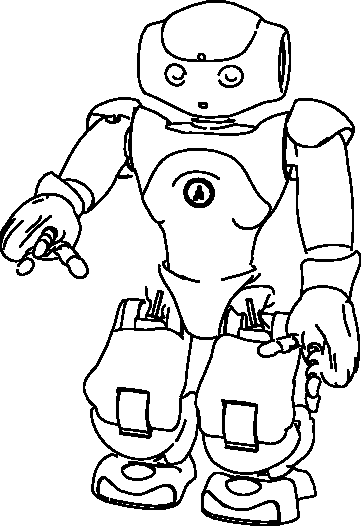
\includegraphics[width=2cm]{nao}};
    \node[below left=2 of laptop] (tablet) {
\includegraphics[width=2cm]{tablet+stylus}};
    \node[above=2 of laptop] (selection) {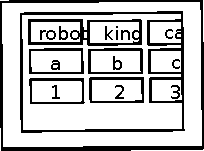
\includegraphics[width=2cm]{selection_tablet}};

    \node[draw,above right=2 of laptop,anchor=north west,text width=4cm] (processes)
    {\sf\scriptsize machine-learning, \\letters/gestures
    generation, \\interaction supervision};
    \path (laptop) edge[dashed] (processes);

    \path (nao) edge [->,redarrow, bend left] node[label, auto] {robot state} (laptop);
    \path (laptop) edge [->,greenarrow, bend left] node[label, auto] {writing gestures} (nao);

    \path (tablet) edge [->,redarrow, bend left] node[label, auto] {demonstrations,\\turn taking} (laptop);
    \path (laptop) edge [->,redarrow, bend left] node[label,
    auto=right,align=right]
    {path of\\ letters to display} (tablet);

    \path (selection) edge [->,redarrow] node[label, auto=right] {letter/word to write} (laptop);

    \path (-5, 2) edge [->, redarrow] node[label] {ROS} ++(1, 0);
    \path (-5, 2.6) edge [->, greenarrow] node[label] {NaoQI} ++(1, 0);
    
\end{tikzpicture}
}

\caption{\small \textbf{Overview of the system}. In total, the system runs about 10 ROS nodes,
    distributed over the robot itself, a central laptop and Android tablets.}

    \label{fig:archi}
\end{figure}

The overall architecture of the system (Figure~\ref{fig:archi}) is therefore
spread over several devices: the {\sc nao} robot itself, that we address via
both a ROS API\footnote{The ROS stack for {\sc nao} is available at 
\url{http://wiki.ros.org/nao_robot}.} and the Aldebaran-provided NaoQI API, one
to four Android tablets (the main tablet is used to print the robot's letter and
to acquire the children's demonstrations; more tablets have been used in some
studies, either to let the child input words to be written, or for the
experimenter to qualitatively annotate the interaction in a synchronized
fashion), and a central laptop running the machine learning algorithms, the
robot's handwriting gesture generation and high level control of the activity.

Since the system does not actually require any CPU-intensive process, the laptop
can be removed and the whole logic run on the robot. Due to the relative
difficulty to deploy and debug ROS nodes directly on the robot, the laptop
remains however convenient during the development phase and we kept using it in
our experiments.

Most of the nodes are written in Python, and the whole source code of the
project will be made is available online\footnote{The primary repository is\\ 
\url{https://github.com/chili-epfl/cowriter_letter_learning}.}.


\section{case study 1: Vincent}\label{Vincent}
\subsection{Context}
Vincent$^*$ is a five year-old child. At school, he has difficulties to learn writing, particularly with cursive letters. From our perspective, Vincent is shy and quiet. He suffers from poor self-confidence much more than any actual writing problem. The experiment was conducted without any therapist, in our laboratory. A parent was here to accompany the child, but she did not intervene during interactions. Children's personalities, conditions and state evaluation were reported by the parent.

\subsection{Hypothesis}

The CoWriter activity needs a child engaged as interaction leader. 
With this study we consider the problem of long-term interactions. We hypothesize that with an appealing scenario children can maintain motivation in doing a handwriting activity for an hour over 4 sessions.

%   \begin{figure}
%       \centering
%       \includegraphics[width=0.9\linewidth]{Vincent_start}
%       \caption{Homework performed by Vincent before the experiment. It gives an
%       overvew of his starting level in handwriting.}
%       \label{fig:Vincent_start}
%   \end{figure}
%
%   \begin{figure}
%       \centering
%       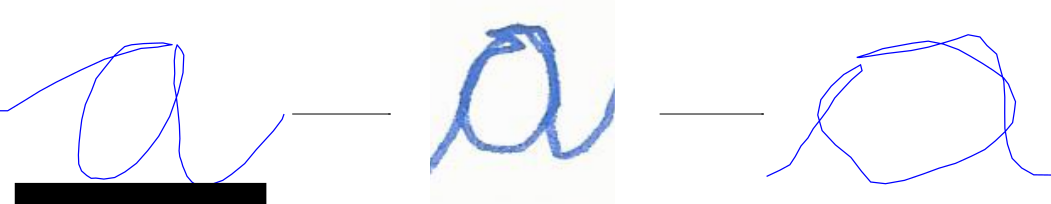
\includegraphics[width=0.9\linewidth]{3a}
%       \caption{Letter deformation along an eigenvector. \emph{Left} : the non-deformed
%           letter (origin of the subspace). \emph{Middle} : the actual Vincent's
%           deformation (from figure~\ref{fig:Vincent_start}). \emph{Right} : exaggerated
%   deformation along the eigenvector that encode Vincent's mistake.} 
%       \label{fig:3a}
%   \end{figure}

\subsection{Experimental design and methodology}

Our goal was to provide Vincent with
an environment that would enable him to sustain engagement over four one-hour sessions, 
one session per week. We decided to introduce a scenario to elicit a strong ``prot\'eg\'e effect" and such induce a stronger commitment. While the child came with low intrinsic motivation in writing exercise, our idea was to use the robot to introduce a new extrinsic motivation: improving letters in order to help the robot. 


In our scenario we used two Nao robots: a blue one 
(called Mimi) and an orange one (called Clem). Mimi was away for a 
scientific mission, and the two robots had to communicate by mails. But they decided to do it 
``like humans", with handwritten messages. While Mimi was good in handwriting, 
Clem had strong difficulties and needed Vincent's help.

Mimi's mission was to explore a mysterious hidden
base. Each week, a postal mail contenting
a picture of a curious object it found and a few handwritten words about its discoveries. 
The picture showed itself exploring 
a dark room of the hidden base (that was actually our laboratory's workshop). 

During the three first sessions, Clem (the robot interacting with the child) was waiting for Vincent
with the received mail. It let Vincent take a look at the picture and the object,
and then it asked him to read the message.
Finally, Vincent formulated a response and helped the robot to write it.

The fourth and last session was set as a test: Mimi, the ``explorer'' robot,
came back from its mission and challenged Clem in
front of Vincent: \emph{``I don't believe you wrote yourself these nice letters that I
received! Prove it to me by writing something in front of me!''} This situation
was meant to confirm the prot\'eg\'e effect: by judging the other robot's
handwriting, Mimi would implicitly judge Vincent's skills as
teacher, and in turn, Vincent's handwriting.

To complement the intrinsic motivation of helping a robot to communicate with another one, we
gradually increased the complexity of Vincent's task to keep it challenging and
interesting (first week: demonstration of single letters; second week:
short words; third week: a full message -- Figure~\ref{fig:stimuli}).
%
%Vincent had to tell the robot what to write with small plastic letters (visible
%behind the robot on Figure~\ref{fig:Vincent}). A third person was here to send
%the formed word to the robot via the computer.

Vincent had to tell the robot what to write with small plastic letters. A third person was here to send
the formed word to the robot via the computer.

During the experiment, all robot and child writings on the tablet were recorded on log files. Likewise, we recorded the time date when the child start and finish a demonstration.  

%\begin{figure}
%    \centering
%    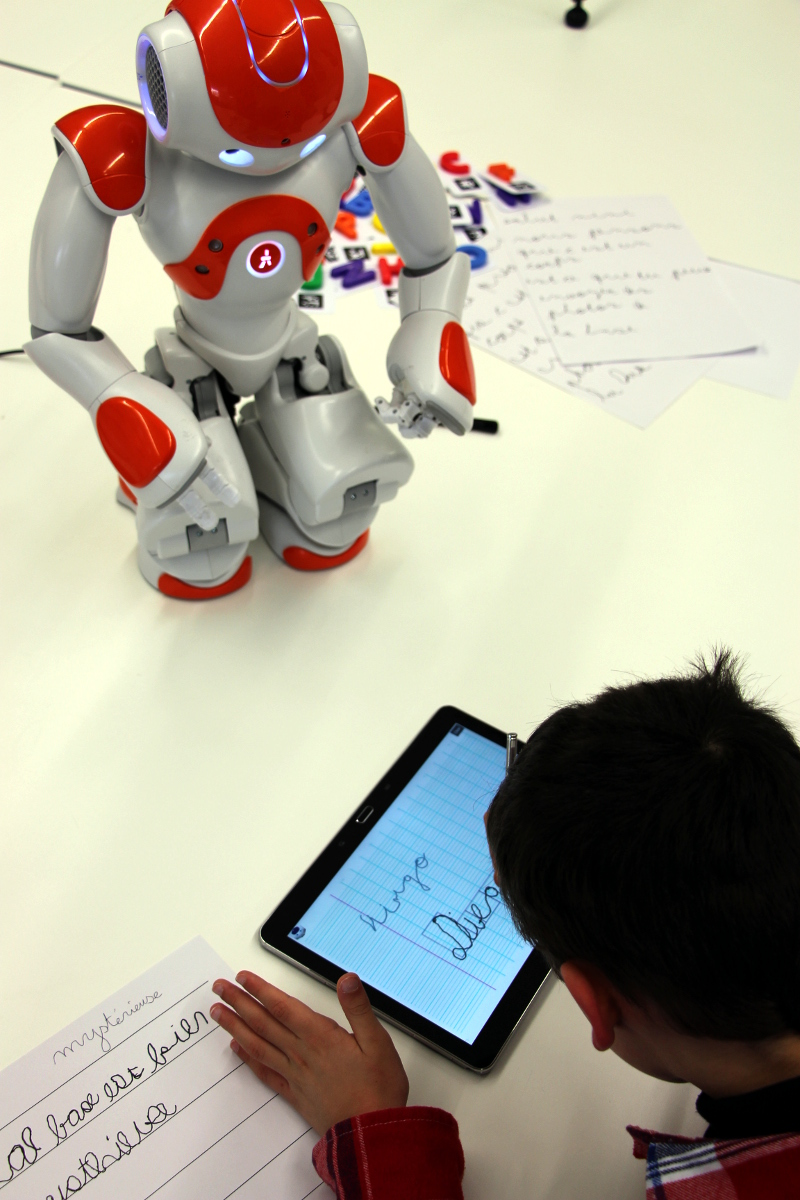
\includegraphics[width=0.4\linewidth]{diego}
%    \caption{\small Vincent correcting {\sc nao}'s attempt by rewriting the
%        whole word. Empty boxes are drawn on the screen to serve as template for the child
%        and to make word segmentation more robust.}
%    \label{fig:Vincent}
%\end{figure}

\subsection{Measures}

%   \begin{figure}
%       \centering
%       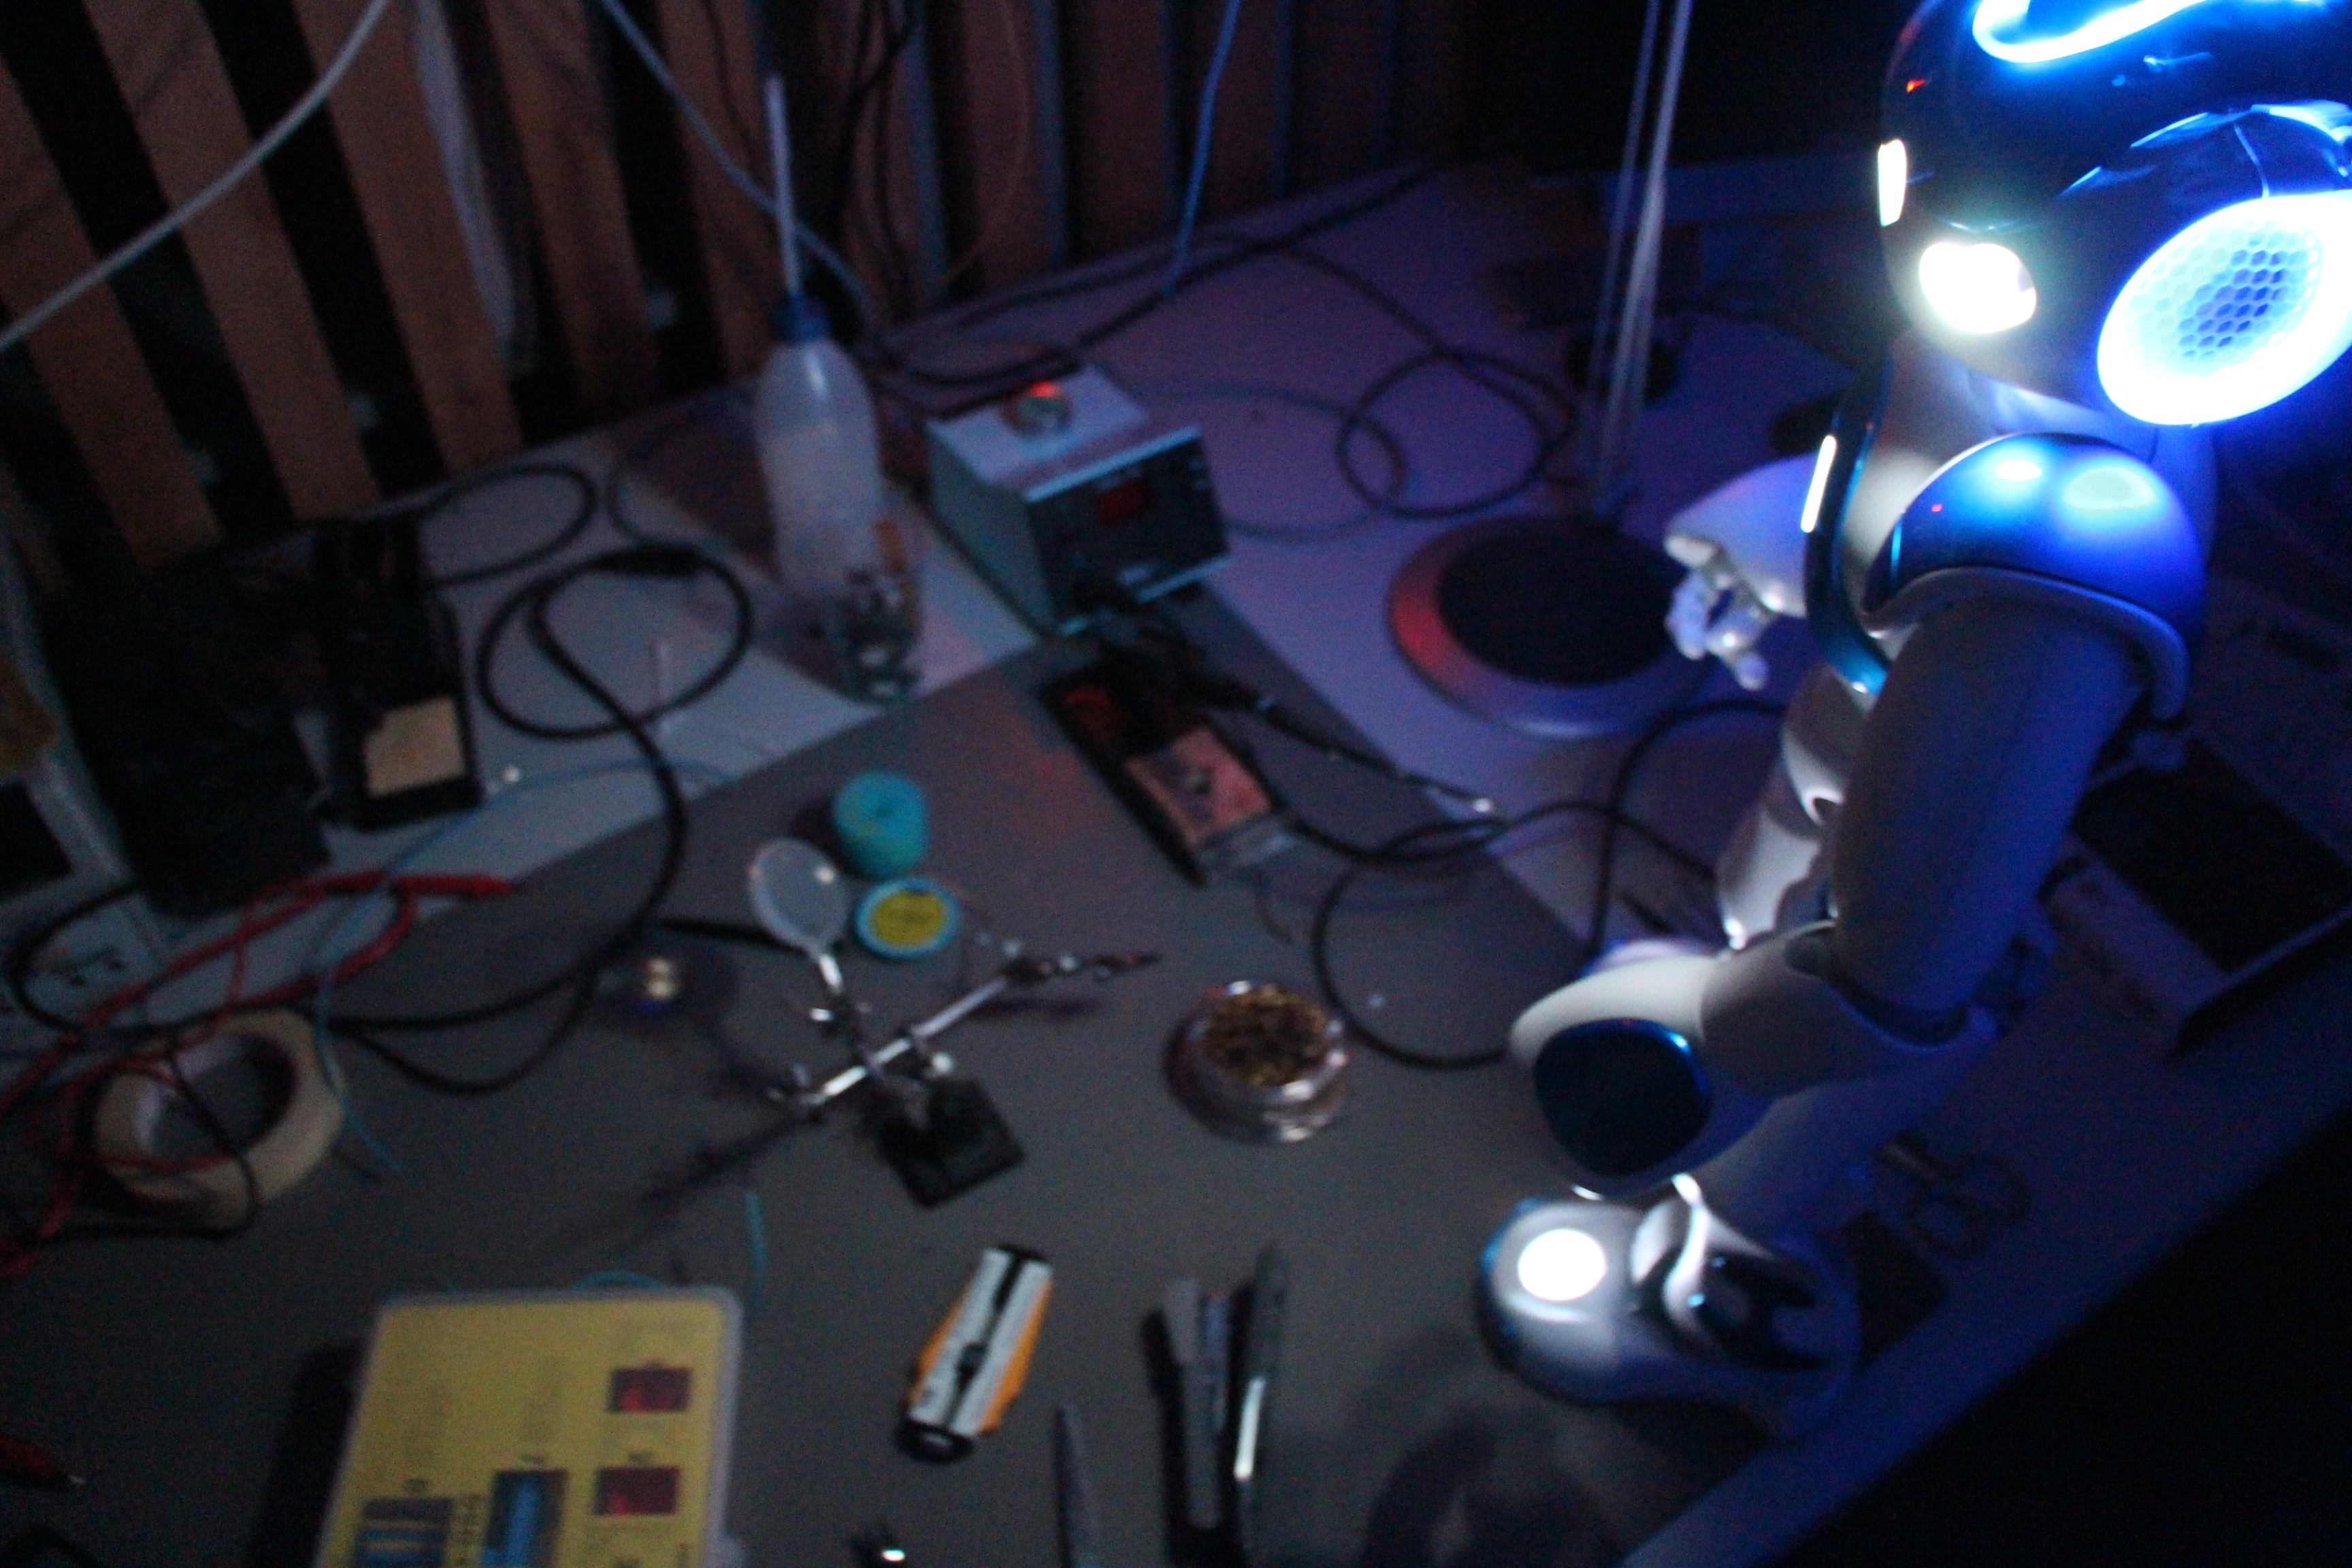
\includegraphics[width=0.9\linewidth]{mimi_mails}
%       \caption{Exemple of content of the mails sent by Mimi. A : pictures of Mimi exploring the
%           hidden base. B : some curious objects found by Mimi in the base. C :
%           few words about its adventures and discoveries.
%       }
%       \label{fig:mimi_mails}
%   \end{figure}
We measured the commitment of the child with the number of demonstration he provided. We also measured the duration of sessions. During the two last sessions, we recorded the time taken by the child to write demonstrations.

After the experiment we interviewed the parent of the child. She was asked if she observed any impact of our activity on the child.


\subsection{Analysis}

We compared the number of demonstrations provided by Vincent along the 4 sessions (reported on Table~\ref{table:vincent_sess}) and we summed the time spend by the child to write demonstration during the 2 last sessions.
\begin{table}
    \centering
    \begin{tabular}{|c|c|c|c|c|}
        \hline
        Session & S1 & S2 & S3 & S4\\ \hline
        Number of demo & 23 & 34 & 52 & 46\\ \hline

    \end{tabular}
    \caption{\footnotesize Number of demonstrations provided by Vincent along the 4 sessions.}
    \label{table:vincent_sess}
\end{table}
\subsection{Results}
Overall, Vincent provided 155 demonstrations to the robot. We can see in Table~\ref{table:vincent_sess} that the number of demonstrations provided by Diego was globally increasing along sessions while the difficulty of the activity was also increasing. Interestingly, as the number of demonstration decreased from session 3 to session 4, the total time spend to write demonstrations is similar: 41.6s in session 3 ($\thicksim$0.8s per letter) and 41.1s in session 4 ($\thicksim$0.89s per letter). A explanation of this result could be that since the difficulty was increasing the child spent more time to write his demonstrations. Our activity succeeded in the sense that the child found enough motivation to provide an increasing number of demonstrations, and was still (or even more) carefully in the last session.

After the first week, he showed
confidence when playing with his ``prot\'eg\'e" and he built affective bonds with the robot
over the course of the study, as evidenced by some cries on the last session,
and several letters sent to the robot \emph{after} the end of the study
(one of them 4 months later) to get news. This represents a promising initial
result: we can effectively keep a child committed into the activity with the robot for a relatively
long periods of time (about 5 hours).

From the parent's perspective, Vincent was actually showing a new motivation in improving his handwriting. He took pleasure to work with the robot and to accomplish his teacher's mission. She confirmed that an affection of the child for the robot took root within the experiment. Finally she saw an improvement of his handwriting and explained that the child ``passed from a mix of script and cursive writing up to a full-cursive writing".

But no conclusion can be drawn in terms of actual handwriting remediation: we did
not design this study to formally assess possible improvements. However, as pictured on Figure~\ref{fig:stimuli}, Vincent was able to
significantly improve the robot's skill, and he acknowledged that he had been
able to help the robot: in that regard, Vincent convinced himself that he was
``good enough'' at writing to help someone else, which is likely to have
a positive impact on his self-esteem.

\begin{figure}
    \centering
    \subfigure[Initial letter, generated by the robot]{
        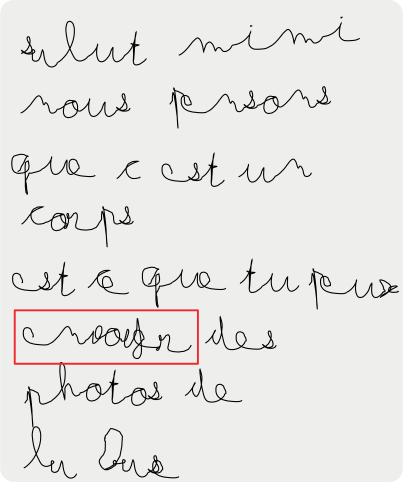
\includegraphics[height=4.5cm]{diego-initial-letter}
    }
    \subfigure[Final letter, after training with Vincent]{
        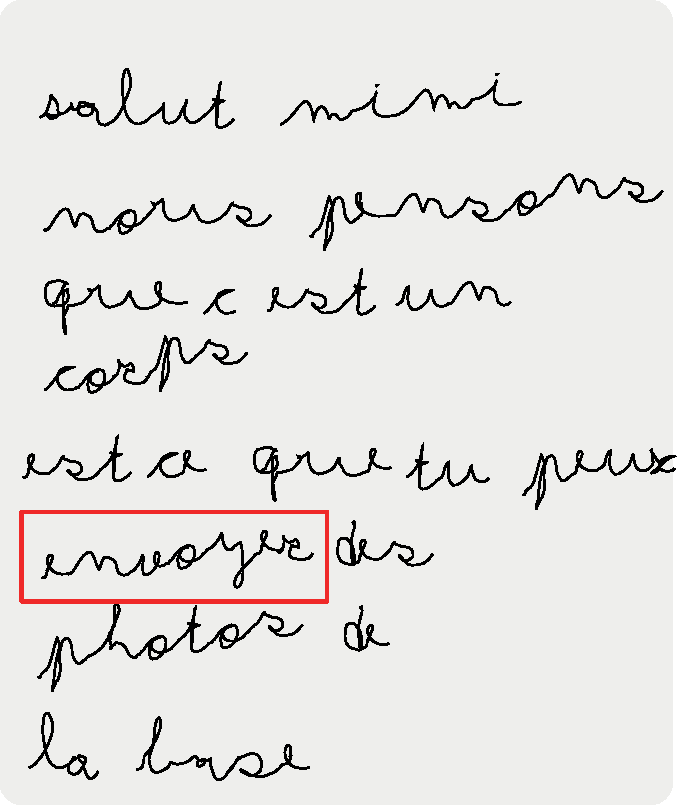
\includegraphics[height=4.5cm]{diego-final-letter}
    }

    \caption{\small (French) text generated by the robot, before and after a one
        hour long interaction session with the child. As an example, the red box
        highlights the changes on the word ``envoyer''.}

    \label{fig:stimuli}
\end{figure}



\section{case study 2 : Thomas}\label{Thomas}

\subsection{Context}

Thomas, 5.5 years old child, is under the care of an occupational
therapist. He has been diagnosed with visuo-constructive deficits.
He was frequently performing random attempts and then was comparing
with the provided template. Thomas is restless and careless: he
rarely pays attention to
advice, even to what he is doing when he is currently drawing, and he is
quickly shifting his attention from one activity to another.

Thomas was working on number allographs with his therapist. During a prior
meeting, the therapist provided us with a sequence of numbers
written by Thomas. one of the observed problems was drawing
horizontally-inverted allographs, mainly for ``5". The experiment was conduced with Thomas' therapist. 

\subsection{Hypothesis}

The CoWriter activity can be adapted to a pedagogical context and help a child with diagnosed deficits to learn handwriting. 

We believe that small modifications of the activity adapted to
Thomas problems (visuo-constructive deficits and inattention) could help to
keep him focused on the activity during forty-minutes sessions, and to evidence to the child that the robot is progressing by dint of his demonstrations. 

\subsection{Experimental design and methodology}
The experiment was conducted in the therapist's office (four sessions 
spanning over 5 weeks). We assumed that a scenario like the one we used 
for Vincent would not be usable with Thomas. We just introduced the robot 
and quickly said that it was seeking help to train for a robot handwriting contest.

In order to integrate our work with that of the therapist, we decided to adapt the 
CoWriter activity to work with numbers.

Since Thomas was frequently drawing horizontally-inverted numbers, or even
unrecognisable allographs, the learning algorithm of the robot was converging to
meaningless scrawls. To fix this problem, we programmed the robot to refuse allographs that
were too distant to a reference with a threshold we arbitrary fixed. In that way,
the child was forced to take care on what he was providing to the robot as
demonstration. 

According to the therapist, it was easier for Thomas to memorize the way to draw
a number if it was always done is the same order, \emph{e.g.} if the ``5" was always
drawn from the top-right tip down to bottom. Therefore we programmed the robot to
refuse as well a good allograph drawn in a wrong order. But in order to reassure Thomas
about the right final allograph's shape, we made the robot able to recognize
such a drawing, and, when it occurred, to use the phrase:
\emph{``Oh, this is exactly the shape of the number I want to learn, but can you
show me how to draw it in the opposite direction?"}

Also, to make
the robot's progresses evident, we modified the initialization step of the
learning algorithm to start with a roughly vertical stroke instead of a
deformed number (round 0 on Figure~\ref{learning_6_demos}).

In this setup, we added a second tablet with one button per number. It was used
by the child to chose a new number to teach to the robot. It also provided the
possibility to enter letters or words, and to switch to another activity (robot telling a story if the child needs a short break).

\subsection{Measures}

We recorded all the demonstration (vector of 70 points) performed by the child and by the robot to study if the child took care of his writing to make his demonstration accepted and if he was actually able to improve the robot's skills given the metric used to accept/reject. 

The duration of sessions and the time spend by demonstration were also recorded by the logs of the tablet. 


\subsection{Analysis}

It was difficult to make comparison between different sessions since the child did not work on the same numbers. But we could study the evolution of the quality of Thomas' demonstration when he was working on a given number (Figure~\ref{Thomas_progress}).
To show how Thomas leaded the robot to reach his level we plotted on the same graph the evolution of the quality of Thomas' demonstrations and the robot's trials (Figure~\ref{Thomas_distances}). We also reconstructed and displayed the drawn allographs of the number 6 to visualize the impact of the lessons of Thomas on the robot (Figure~\ref{learning_6_demos}). 

\begin{figure}
    \centering
    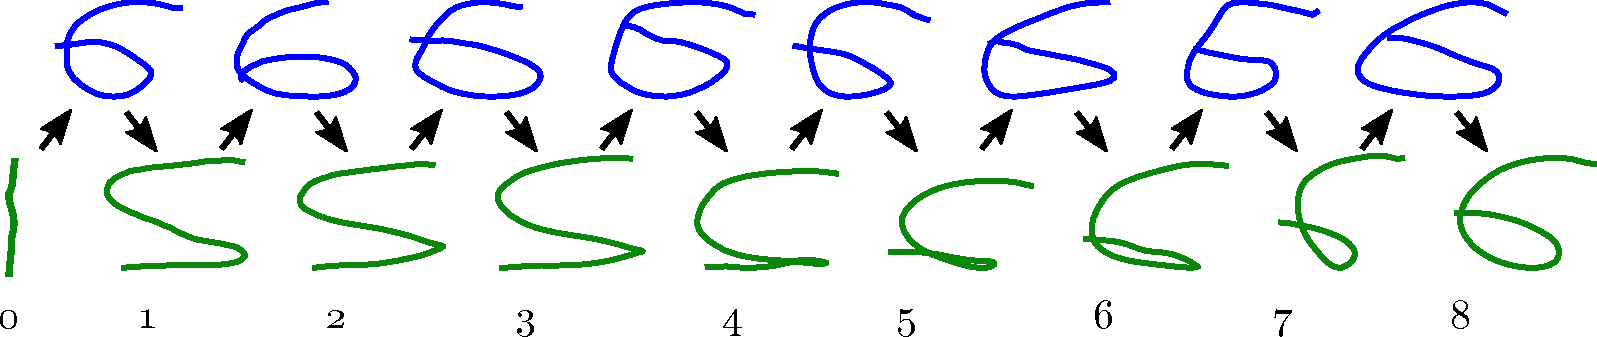
\includegraphics[width=0.9\linewidth]{learning_6_demos}
    \caption{\small Demonstrations provided by Thomas for the number ``6'' (top row) and
        corresponding shapes generated by the robot. After eight demonstrations,
        Thomas decided that the robot's ``6'' was good enough, and went to
    another character: in that respect, he was the one leading the learning
process of the robot.}
    \label{learning_6_demos}
\end{figure}

\subsection{Results}
Despite his attention deficit, Thomas was able to remain engaged in the activity during more than
forty minutes in each session. In total, 55 allographs out of 82 
demonstrated by the child were acceptable considering our threshold (with a
progressive improvement from 13 out of 28 in the first session up to 26 out
of 29 in the last session).

As soon as Thomas understood that the robot was only accepting well-formed
allographs, he started to focus on it and he would typically draw 5 or 6 times
the number before actually sending to the robot (the tablet lets children
clear their drawing and try again before sending it). According to
the therapist, it was the first time that Thomas would correct himself in such a
way, explicitly having to reflect on how \emph{another agent} (the robot) would
interpret and understand his writing. Figure~\ref{Thomas_progress} shows how
he gradually improved his demonstrations for some numbers, according to the
metric we used to make the robot accept/refuse samples.

Since the robot's handwriting started from a simple primitive (a stroke), each
time Thomas succeeded to have his demonstrations accepted by it, the robot's
improvement was clearly visible (as measured in Figure~\ref{Thomas_distances}).
This led to a self-rewarding situation that effectively supported Thomas'
commitment.

\begin{figure}
    \centering
    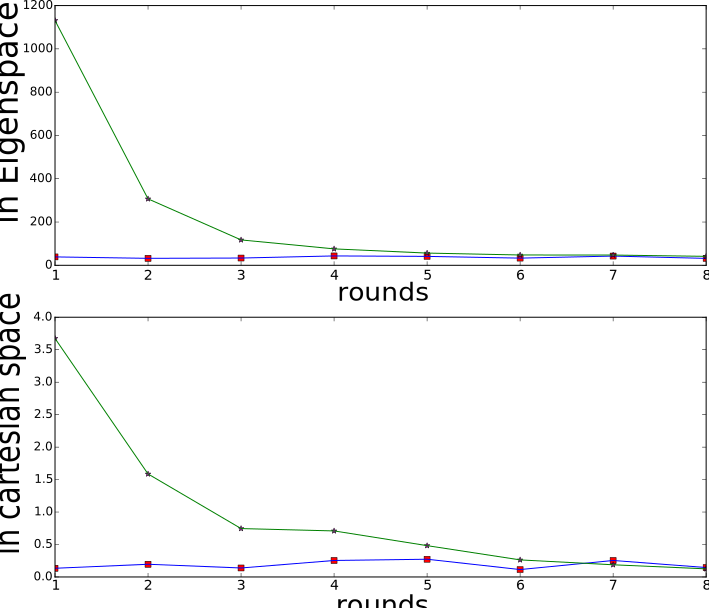
\includegraphics[width=0.9\linewidth]{learning_6_distances}
    \caption{\small Two metrics to assess the handwriting progresses: Euclidean
    distance in the subspace of the number dataset (top figure) or in
Cartesian space (bottom figure). Green lines represent the robot performance,
blue lines performance of the child. The round IDs correspond to the demonstrations
pictured on Figure~\ref{learning_6_demos}.}
    \label{Thomas_distances}
\end{figure}

%\begin{figure}
%    \centering
%    \includegraphics[width=0.9\linewidth]{learning_6_progress}
%    \caption{\small .}
%    \label{Thomas_progress}
%\end{figure}

\begin{figure}
    \centering
    \subfigure[number 2]{
        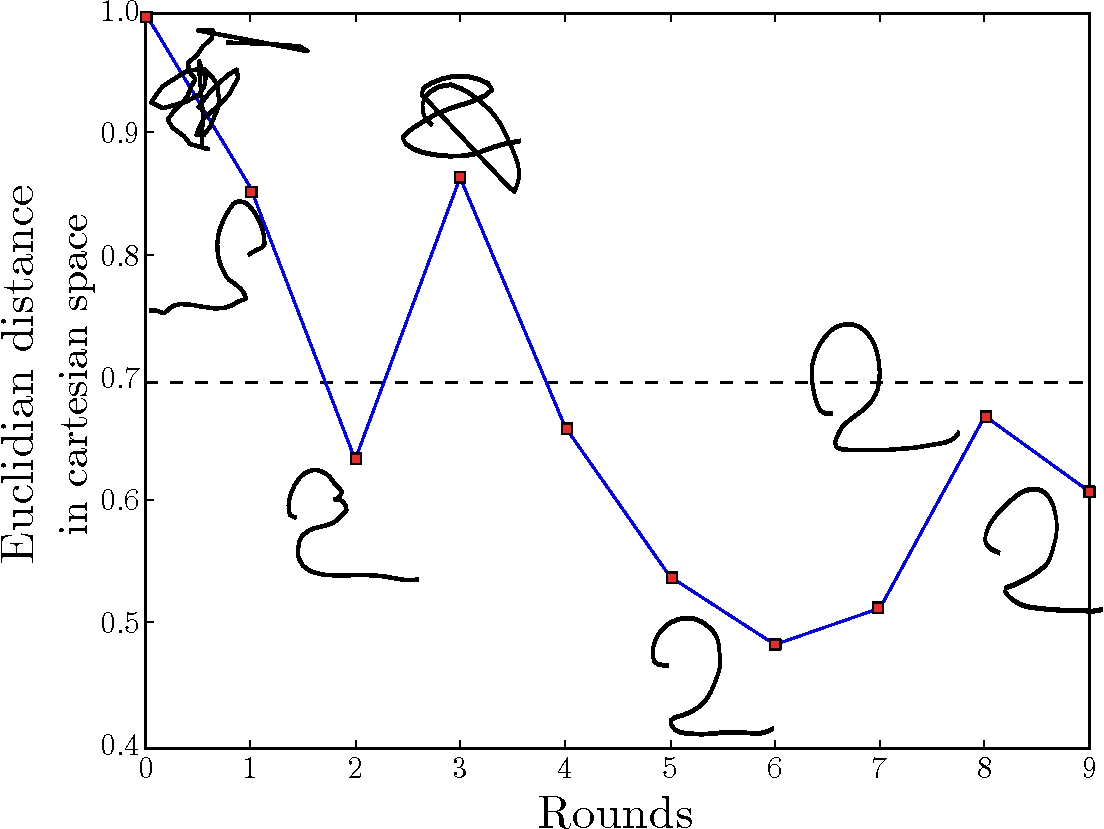
\includegraphics[width=4.1cm]{henry2}
    }
	\subfigure[number 5]{
        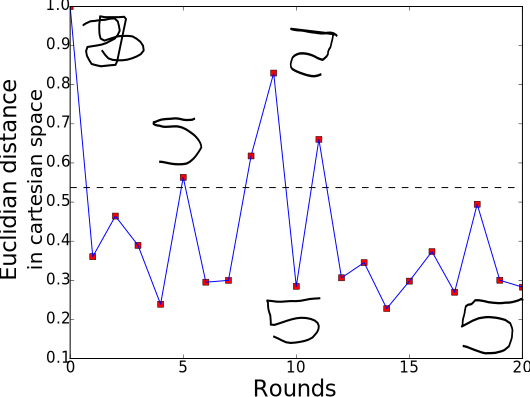
\includegraphics[width=4.1cm]{henry5}
    }
    \caption{\small Improvement of Thomas demonstrations for some numbers: a) the number 2 and b) the number 5. Thomas progressively took care of the demonstrations he was providing to the robot for those numbers. We used for this figure the same metric than the one used for the acceptance algorithm. Distances are normalized with respect to the biggest value. The dashed line correspond to the threshold of robot's acceptance.}

    \label{Thomas_progress}
\end{figure}

\section{Case study 3: when children evaluate the robot}\label{auto}

\subsection{Context}

Each of previous studies was adapted to individual subjects : we used a special
design for each case in order to sustain the child's commitment.
In our next experiment, we conducted case studies with eight children using a single design. These children have in common difficulties to learn
cursive writing but the natures and intensities of those troubles are radically
different from one child to another. Valerie (7 years old), Antoine (6.5) and
Johan (7) are under the care of an
occupational therapist. Emilien (8) and Mathieu (7) are repeating their school year
because of writing. Marie (6) and Adele (8) are bottom of their respective
classes in writing activities. Nicolas (7) is under the care of a neurologist, and
has been diagnosed with specific language impairment. All of these children are
expected, given their school level, to know the allographs of
cursive letters. The experiment was conducted along with an ergotherapist. 

Our goal was to study the perception of the robot's progress in children. We want to know how easily they are able to take the role of teachers and to detect improvements or eventual degradations of the robot's letters. 


\subsection{Hypothesis}

Children understand they role and find motivation to teach the robot. They are able to perceive robot's progress, and evaluate it in correlation with its progress in handwriting.

\subsection{Experimental design and methodology}

This experiment took place in the coffee room of a therapists shared surgery
in Normandy, France. Over two weeks, each child came three times for one-hour
session, except Adele and Marie who did just one session. A facilitator was present to explain the rules of the game and tablet usage. As in the previous experiment, children were provided with two tablets : one to choose a word (or a single letter) to teach, and one
used by both the child and the robot to write. We also provided the allograph's template if the child asked for. 

The starting point of the robot's writing was the same for all children: we
used middle point between simple vertical strokes and letters. For this study,
we wanted the robot to be only influenced by the demonstrations provided by the
child, so we did not project allographs in a subspace. The new generated
sample by the robot were calculated as the middle way between demonstration and
last state in Cartesian space. 

The robot was programmed to accept all demonstrations, giving to the child the
full responsibility of the teacher.

We added two buttons on the tablet  interface: a green one with a ``thumbs up", and
a red one with a ``thumbs down". Those buttons could be used by children to evaluate the
robot (the green one was for rewards while the red one was for punishment). This
way, we could measure the perception of the robot by the child: the more the
child used evaluation buttons, the more he was playing the teacher, judging the
robot instead of himself. Children were free to use the buttons when they wanted during the experiment. 


\subsection{Measures}

As in previous studies, we recorded the times of all demonstrations, the duration of demonstrations and we measured the commitment as the number of demonstration per session. 
We recorded in logs each time an evaluation was provided by children. The awareness of children for the robot progress is measured as the correlation between children evaluations and distances between robot's letters and optimal templates.

\subsection{Analysis}

Since sessions took place over only two weeks, we did not studied possible
handwriting remediation in children, but we focused on correlation between the children's evaluations and the robot's progression.
We estimated the robot's progression as the difference between a starting score
(score of the first robot's try when children have chosen a new word/letter to
work on) and the current robot's score (after being taught by the child). The
score is calculated as the average of euclidean
distance between robot's try and a reference allograph over all letters of the
word. Those references for letter allographs where drawn by us beforehand, taking inspiration in education.com cursive letters template\footnote{\url{http://www.education.com/slideshow/cursive-handwriting-z/}}. For each trial of the robot, we associate two values: the score of progress, and the child's immediate feedback (+1 if the child pressed the green button, -1 if he pressed the red one, 0 if he did not pressed any button after the trial). Then we focused on trials associated with non-zero grades and established Pearson's correlation test between score of progress and children feedback.

\subsection{Results}

All children maintained their engagement during the whole sessions. They provided
on average 42 demonstrations per session. All children used evaluation buttons and
had preference to reward the robot (in total, 99 rewards and 33 punishments were recorded). Interestingly, the time spent by children to write one demonstration systematically increased from one session to the following. We can interpret this phenomena by the fact that they were more careful to slowly explain the correct gesture to the robot. 

We found that 5 of the 8 children provided evaluation significantly correlated with robot's progress. The coefficients of correlation and p-values of each child is reported in the second-to-last column of Table~\ref{table:scores}.

We also studied correlation between children's evaluations and their own
progression. The analysis was conducted in the same way, using distances between children demonstrations and reference allographs to compute children progressions.
3 of 5 children evaluations correlated with the robot's progress were also significantly correlated with their own progress (last column of Table~\ref{table:scores}). For
those children, it seems that the robot was reflecting their own performances, and while they
were judging the robot positively (three times more rewards than punishments)
they were actually evaluating themselves.


\begin{table}
    \centering
    \begin{tabular}{ccccll}
        \toprule
        \bf Child      & \bf \# Dem & \bf \# Pos & \bf \# Neg & $r$ (robot) & $r$ (child) \\ \midrule
        \emph{Val\'erie} & 42           & 24              & 6               & 0.25 \small\tt ** & 0.14 \small\it ns\\ 
        \emph{\'Emilien} & 74           & 20              & 9               & 0.06 \small\it ns & 0.02 \small\it ns\\
        \emph{Mathieu} & 43           & 10              & 3               & 0.23 \small\tt ** & 0.21 \small\tt **\\
        \emph{Nicolas} & 38           & 16              & 4               & 0.31 \small\tt *** & 0.20 \small\tt **\\
        \emph{Johan}   & 32           & 10              & 5               & 0.10 \small\it ns & 0.03 \small\it ns\\
        \emph{Antoine} & 27           & 10              & 3               & 0.20 \small\tt * & -0.02 \small\it ns \\
        \emph{Ad\`ele}   & 35           & 4               & 2               & 0.28 \small\tt * & 0.30 \small\tt ** \\
        \emph{Marie}   & 40           & 5               & 1               & -0.02 \small\it ns & 0.13 \small\it ns\\ \bottomrule
    \end{tabular}
    \caption{\footnotesize Feedback from the children to the robot. \emph{\#Dem}
        denotes the average number of demonstrations per session provided by the children;
        \emph{\#Pos} and \emph{\#Neg} the total number of positive (resp.
        negative) feedbacks they provided. $r$ (robot) and $r$ (child) is the correlation coefficient
        between the feedback provided by the children and the performance of the
        robot (resp. the child himself).}

    \label{table:scores}
\end{table}



\section{Conclusion}
This paper provides the first results of long-term experiments 
with CoWriter activity performed by one child at the time.

Through adaptations of
the interaction design and the learning algorithm, our goal was to induce a prot\'eg\'e effect in order to create an new extrinsic motivation.

The first case studies implied that it was possible to conduct a long-term interaction with the child and the robot keeping the quality of the child's commitment. According to our observations and interviews, we succeeded to induce a prot\'eg\'e effect, by building an affective bond between the child and the robot. We deduced the commitment from the increasing number of demonstrations and time spent to write demonstrations.

In the second study, we showed that the activity can be adapted to therapeutic contexts, and that even a child with strong inattention can find motivation to train the robot. 

The third study aimed to estimate how children understood their role of teacher and how they perceived the robot's progress. We added two buttons to allow children to evaluate the robot. This evaluation was used to measure the comprehension of the child. If all children appeared intrinsically motivated by the activity, we can assume that those who understood and well played their role of teacher (given our measure) found their motivation by playing this role. In that case, since the evaluation was mostly positive, we believe that we successfully induced a prot\'eg\'e effect and that this effect was the key of children's motivation and commitment. 


The evaluation of the robot by the child also provided information about his satisfaction of the
learning process (both the robot's ability to learn and the child's own
ability to teach). We believe that this information could be taken into account by
the robot in order to improve the quality of the interaction. As an example, it
could be used at two levels: $\bullet$ it is possible to detect if the child is playing
seriously or not (a non-serious child may provide unrecognisable drawings and gives good grades to
the robot while its level decreases), or if the child did not understand the
activity (if he never uses the evaluation buttons and spends a lot of time to
give a response). $\bullet$ We can reinforce the learnt allograph when the robot
receives a good evaluation, or make it forget the allograph when it
receives a bad evaluation.

After all these
experiments, we now have a large database of children writings that could be
used to generate more interesting subspaces by PCA and robot initial states. 
Recurrent neural networks (RNN) for handwriting recognition and generation~\cite{DBLP:journals/corr/Graves13} could also be used to generate 
children-like handwriting.

%\section*{Acknowledgments}

%This research was partially supported by the Funda\c{c}\~{a}o para a Ci\^{e}ncia
%e a Tecnologia (FCT) with reference UID/CEC/ 50021/2013, and by the Swiss
%National Science Foundation through the National Centre of Competence in
%Research Robotics.

\bibliographystyle{IEEEtran}
\bibliography{cowriter} 

\end{document}
